\begin{figure}
    \centering
    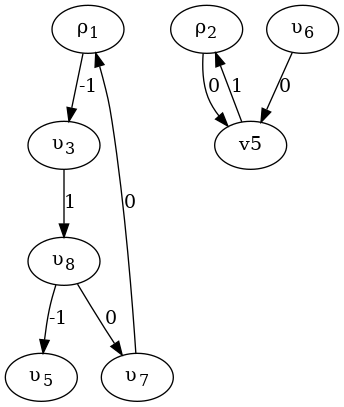
\includegraphics[width=0.3\linewidth]{figures/digraph.png}
% Generating the graph requires \usepackage{dot2texi} or \usepackage[pdf]{graphviz}
%\begin{dot2tex}[file=cstrnts,scale=0.6]
%digraph D {
%    p1 [label=<&rho;<SUB>1</SUB>>];
%    p2 [label=<&rho;<SUB>2</SUB>>];
%    v3 [label=<&upsilon;<SUB>3</SUB>>];
%    v4 [label=<&upsilon;<SUB>5</SUB>>];
%    v6 [label=<&upsilon;<SUB>6</SUB>>];
%    v7 [label=<&upsilon;<SUB>7</SUB>>];
%    v8 [label=<&upsilon;<SUB>8</SUB>>];
%    v7 -> p1 [label="0"];
%    v8 -> v7 [label="0"];
%    p2 -> v5 [label="0"];
%    v6 -> v5 [label="0"];
%    v8 -> v4 [label="-1"];
%    v3 -> v8 [label="1"];
%    p1 -> v3 [label="-1"];
%    v5 -> p2 [label="1"];
%}
%\end{dot2tex}
\caption{Example stage variable constraints as a weighted directed graph}
\label{fig:digraph}
\end{figure}